
\documentclass[11pt,a4paper,openany]{report}
\usepackage[T1]{fontenc}
\usepackage[utf8]{inputenc}
\usepackage{lmodern}
\usepackage{microtype}
\usepackage{amsmath,amssymb,amsthm,mathtools,bm}
\usepackage{booktabs,array,longtable,tabularx}
\usepackage{xcolor}
\usepackage[margin=22mm,headheight=23pt]{geometry}
\usepackage{enumitem}
\usepackage{fancyhdr}
\usepackage{fancyvrb}
\usepackage{graphicx}
\usepackage{url}
\usepackage{xurl}
\usepackage{hyperref}
\definecolor{finblue}{HTML}{1F5A99}
\definecolor{fingreen}{HTML}{19733A}
\definecolor{finorange}{HTML}{D55E00}
\definecolor{finred}{HTML}{A61B1B}
\definecolor{finviolet}{HTML}{6A3D9A}
\definecolor{fingray}{HTML}{4D4D4D}

\hypersetup{
  unicode=true,colorlinks=true,linkcolor=finblue,citecolor=fingreen,
  urlcolor=finblue,
  pdftitle={Nadsoliton Puzzle Atlas: Z12 Audit and Dynamic Reduction},
  pdfauthor={Krzysztof Żuchowski},
  pdfsubject={Controlled cross-disciplinary FIN analysis, Z12 simulator audit, and a theorem on memory generated by dynamic Schur reduction},
  pdfkeywords={FIN, Z12, spectral graph, Schur complement, memory kernel, Mori-Zwanzig, chirality, operator theory}
}
\pagestyle{fancy}
\fancyhf{}
\fancyhead[L]{\small Nadsoliton Puzzle Atlas}
\fancyhead[R]{\small Release 10.22 --- English edition}
\fancyfoot[C]{\thepage}

\setlength{\parindent}{0pt}
\setlength{\parskip}{0.55em}
\setlist{nosep,leftmargin=2em}
\setcounter{tocdepth}{2}
\setcounter{secnumdepth}{3}
\emergencystretch=3em
\newcommand{\one}{\bm 1}
\newcommand{\C}{\mathbb C}
\newcommand{\R}{\mathbb R}
\newcommand{\Z}{\mathbb Z}
\newcommand{\statusProven}{\textcolor{fingreen}{[Proven]}}
\newcommand{\statusStrong}{\textcolor{finblue}{[Strong evidence]}}
\newcommand{\statusModerate}{\textcolor{finviolet}{[Moderate evidence]}}
\newcommand{\statusWeak}{\textcolor{fingray}{[Weak evidence]}}
\newcommand{\statusSpeculative}{\textcolor{finorange}{[Speculative]}}
\newcommand{\statusRefuted}{\textcolor{finred}{[Refuted]}}

\begin{document}
\hypersetup{pageanchor=false}
\begin{titlepage}
\centering
\vspace*{12mm}
{\Large\bfseries FIN --- Release 10.22\par}
\vspace{12mm}
{\Huge\bfseries Nadsoliton Puzzle Atlas\par}
\vspace{6mm}
{\Large Z12 Simulator Audit, Controlled Cross-Disciplinary Intuition,\\
and a New Memory Object after Reduction\par}
\vspace{18mm}
{\Large Krzysztof \.Zuchowski\par}
\vspace{2mm}
{\normalsize Independent Researcher --- Fractal Information Theory Project\par}
\vspace{2mm}
{\normalsize ORCID: \href{https://orcid.org/0009-0002-0909-3613}{0009-0002-0909-3613}\par}
\vspace{10mm}
{\large 28 July 2026\par}
\vfill
\begin{minipage}{0.89\textwidth}
\small
\textbf{Central result.} Exact elimination of hidden strict \(Z_{12}\) nodes
generates a frequency-dependent self-energy and a process with memory.
The static Schur complement is only a resolvent limit, not the exact generator
of the complete reduced dynamics.

\medskip
\textbf{Boundary.} The result does not generate a selector, physical units,
a legacy--strict bridge, or experimental validation.

\medskip
\textbf{Repository.}
\url{https://github.com/hyconiek/Fractal-Nadsoliton-Theory}

\textbf{License.} CC BY 4.0.
\end{minipage}
\vfill
\end{titlepage}
\hypersetup{pageanchor=true}
\pagenumbering{roman}
\tableofcontents
\clearpage
\pagenumbering{arabic}

\chapter*{Confidence convention}
\addcontentsline{toc}{chapter}{Confidence convention}

\begin{itemize}
\item 
\textbf{\statusProven{}} --- an algebraic or numerical result with an explicit test and tolerance.

\item 
\textbf{\statusStrong{}} --- stable in the declared test class, but not a general theorem.

\item 
\textbf{\statusModerate{}} --- a meaningful mechanism with unresolved identifiability.

\item 
\textbf{\statusSpeculative{}} --- a research hypothesis, not a claim about nature.

\item 
\textbf{\statusRefuted{}} --- a claim falsified in the declared model.

\end{itemize}

\chapter{Executive verdict}

The most productive "assembly of the puzzles" does not yield a new scalar parameter or a hidden selector. It yields the operator-valued object

\[
\Sigma_E(z)=A_{EH}(zI+A_{HH})^{-1}A_{HE},
\]

the frequency-dependent \textbf{self-energy of the reduced process}, obtained after partitioning the nodes into observed \(E\) and hidden \(H\) sectors. \textbf{\statusProven{}}

This object unifies five previously separate pictures:

\begin{enumerate}
\item 
Green function/\allowbreak{}resolvent, through the exact block-resolvent formula;

\item 
Schur compression, as the static limit \(\Sigma_E(0)\);

\item 
wave and diffusion dynamics, through the same analytic resolvent family;

\item 
memory and environment, through an exact time-domain memory kernel;

\item 
the observer, as an explicitly supplied accessible/\allowbreak{}hidden partition rather than a metaphysical component of the equation.

\end{enumerate}

It does not solve the three principal omissions of FIN: it does not select an orientation, generate a physical unit, or provide an experimental preparation and apparatus. \textbf{\statusProven{}}

The deepest intuition supplied by the atlas is therefore:

\begin{quote}\itshape
Fractal reduction should not be modeled solely as a static transformation of one kernel into another. Exact elimination of an information level generates a process with memory. The static Schur complement is only its zero-frequency shadow.

\end{quote}

This is a known reduction mechanism in mathematical physics, but its concrete form for the strict FIN operator and its relation to wave--diffusion duality provide a new testable direction inside the project. It is not evidence of new physics.

\chapter{Method: intuition with safeguards}

"Intuitive" comparison can easily turn graphical resemblance into false equivalence. The atlas therefore uses four layers:

\begin{enumerate}
\item 
\textbf{Shape layer:} identify similar plots, symmetries, flows, and diagrams.

\item 
\textbf{Mechanism layer:} determine whether both structures use the same algebraic operation.

\item 
\textbf{Prediction layer:} ask whether the analogy produces a new computable and falsifiable quantity.

\item 
\textbf{Assumption-debt layer:} list everything that must be added before the analogy becomes a physical model.

\end{enumerate}

Each match receives one of five classifications:

\begin{itemize}
\item 
\textbf{exact equivalence} --- an explicit operation-preserving map exists;

\item 
\textbf{common mechanism} --- the operation is shared but the objects or interpretations differ;

\item 
\textbf{structural analogy} --- similar geometry or spectrum without an equivalence theorem;

\item 
\textbf{metaphor} --- visually useful, with no evidential force;

\item 
\textbf{anti-analogy} --- the resemblance exposes the precise point at which FIN differs from the comparison theory.

\end{itemize}

The script fin\_nadsoliton\_puzzle\_atlas.py scanned:

\begin{itemize}
\item 
12 individual characteristics against 15 fields: \textbf{180 comparisons};

\item 
all unordered pairs of characteristics: \(\binom{12}{2}=66\);

\item 
every pair against 15 fields: \textbf{990 comparisons}.

\end{itemize}

This yields \textbf{1170 explicit similarity indices}. Tag-based scoring is only a candidate-search device. It is not evidence and never raises the confidence status of a hypothesis.

\begin{figure}[htbp]
\centering
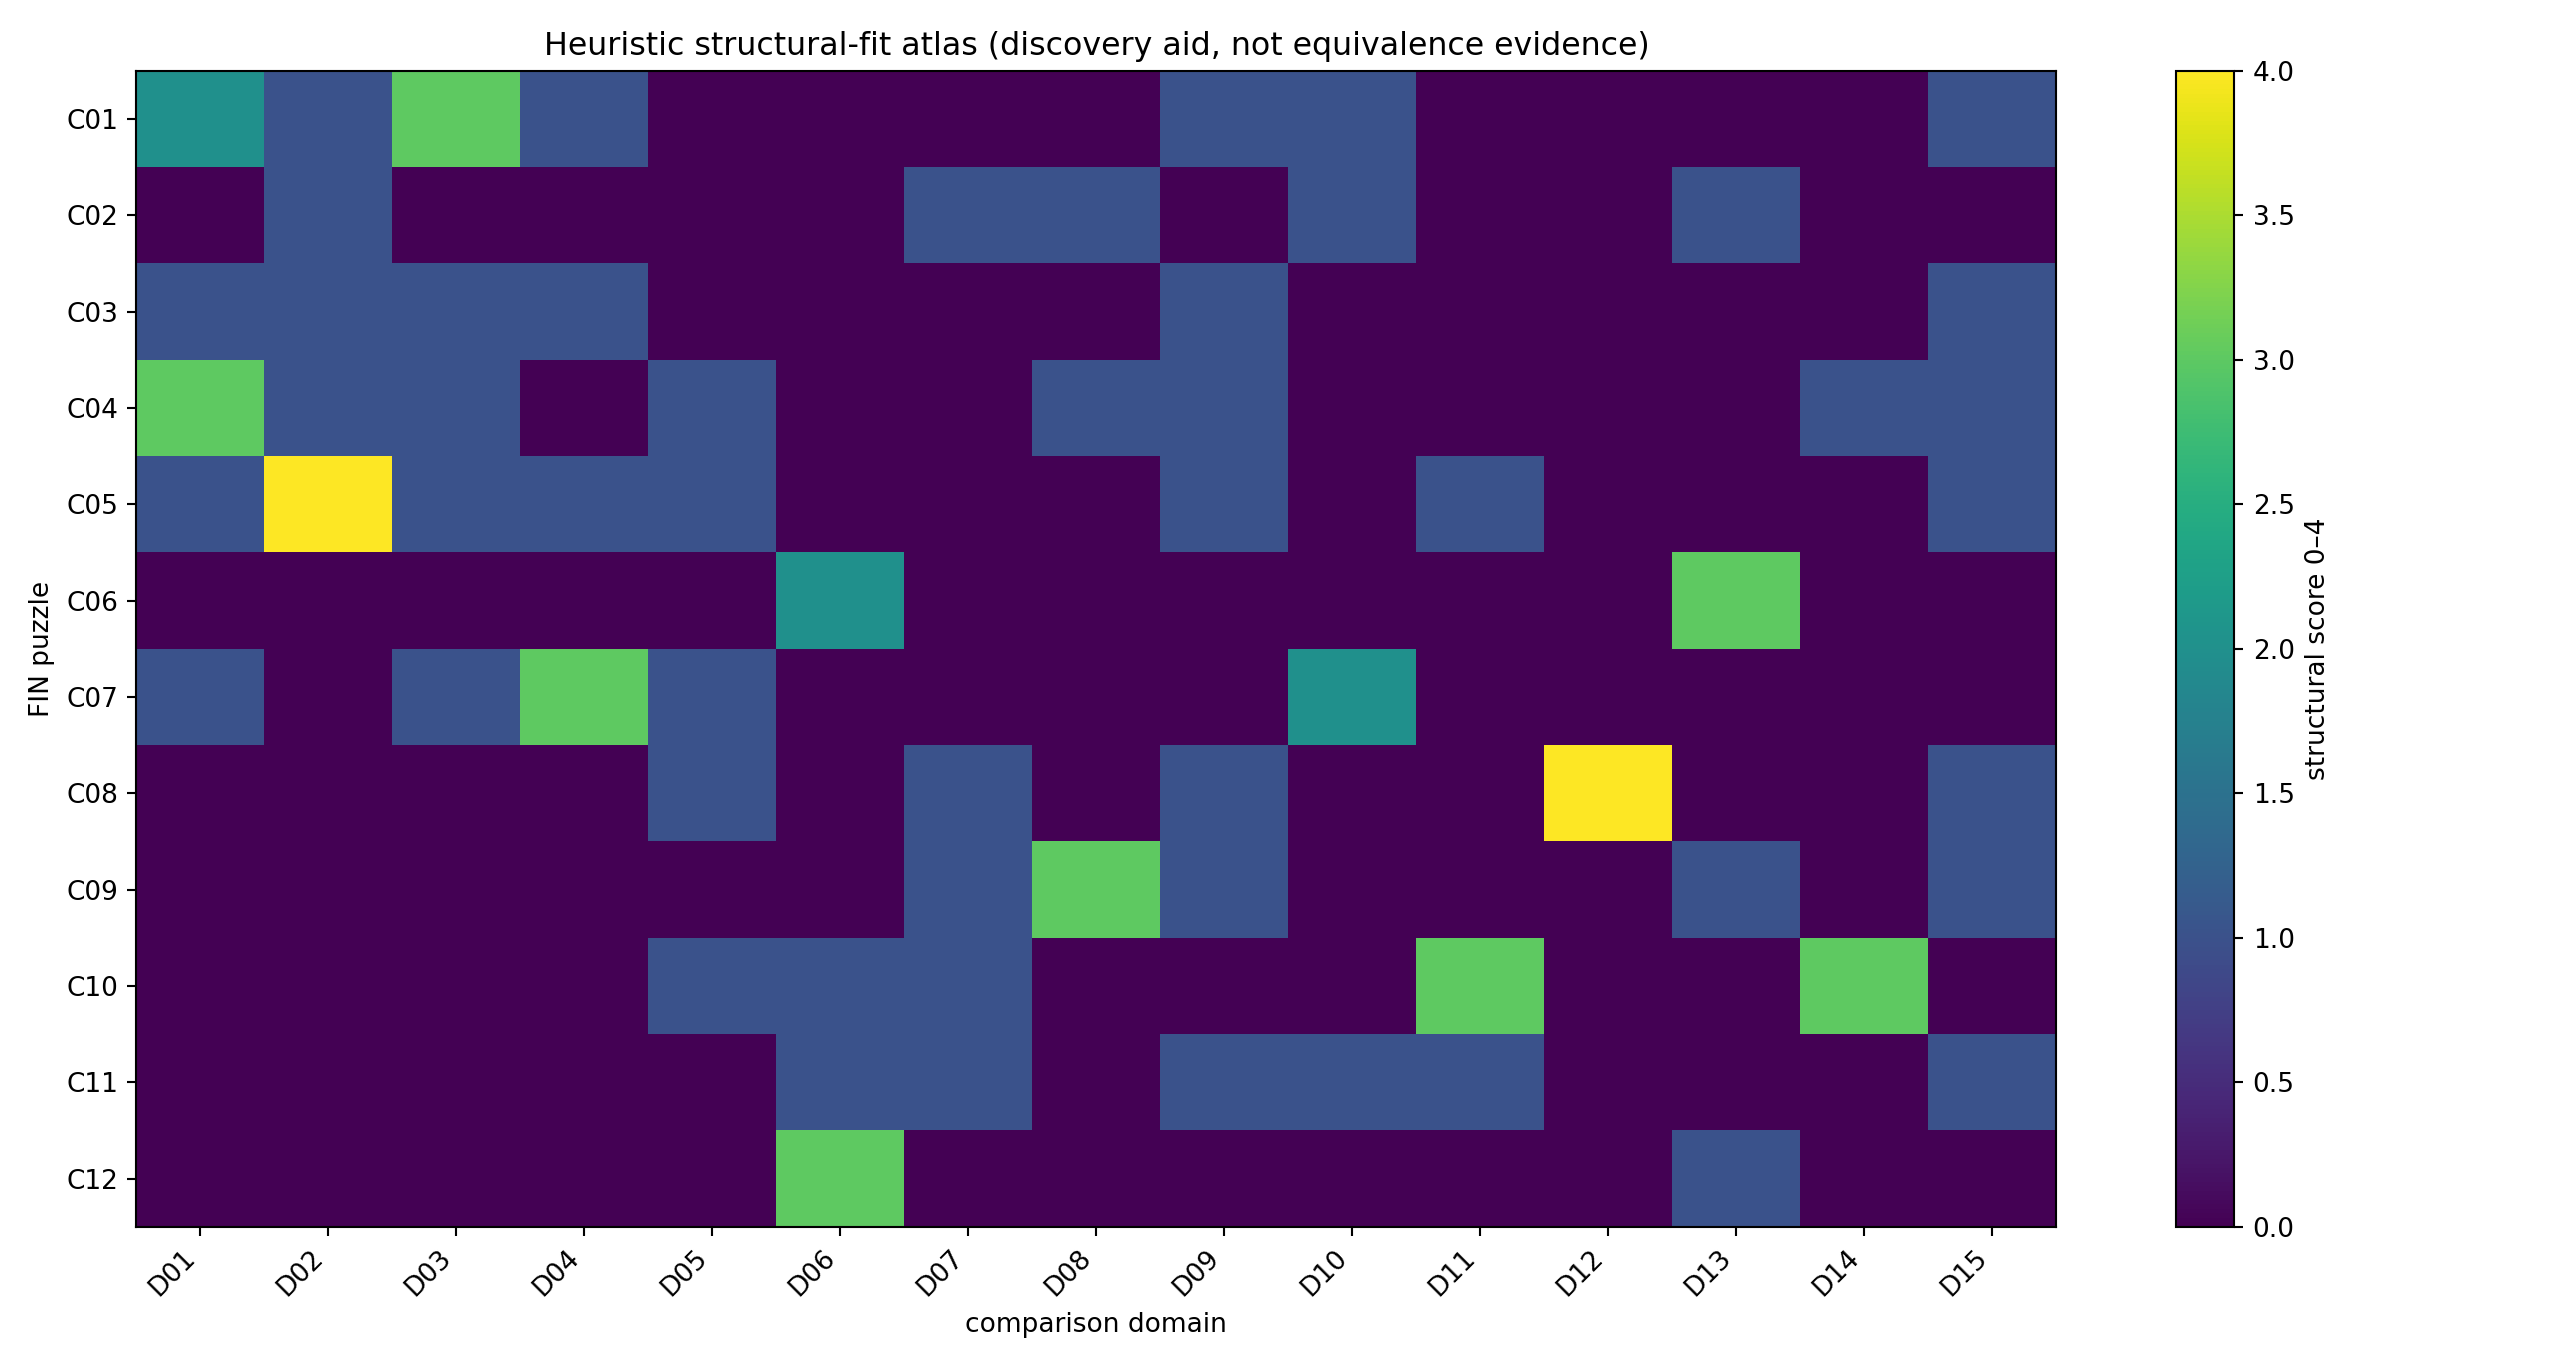
\includegraphics[width=0.97\textwidth]{FIN_Nadsoliton_Puzzle_Atlas_Figures/single_puzzle_domain_atlas.png}
\caption{Heuristic matching matrix for 12 puzzles and 15 fields. Scores are used only to search for analogies.}
\end{figure}

\chapter{What Z12 sim.html actually does}

The code implements a finite thought experiment on \(Z_{12}\):

\[
W_{xy}=K(d(x,y)),\qquad
A=sI-W,\qquad
U_t=e^{-itA}.
\]

The initial state is a partially coherent preparation on two nodes:

\[
\rho_0(\phi,\eta)
=\frac12\Big(
|a\rangle\langle a|+|b\rangle\langle b|
+\eta e^{-i\phi}|a\rangle\langle b|
+\eta e^{i\phi}|b\rangle\langle a|
\Big).
\]

After the evolution \(\rho_t=U_t\rho_0U_t^\dagger\), the code evaluates

\[
p_x(t)=(\rho_t)_{xx},
\qquad
J(x\to y)=2W_{xy}\operatorname{Im}(\rho_{yx}),
\]

and two different aggregate current observables:

\[
C_1=\sum_xJ(x\to x+1),
\]

\[
C_\chi=\sum_x\sum_{d=1}^{5}d\,J(x\to x+d).
\]

\(C_1\) sees only the first hop harmonic. \(C_\chi\) is an oriented group current of the full kernel, excluding the antipodal edge \(d=6\), because a sign cannot be assigned to the shortest displacement there without an additional convention.

The simulator's intended distinction is sound: a \textbf{sign receiver} is not a \textbf{sign source}. A radial operator can transport prepared chirality into a measurable current, but it does not choose the sign of the phase.

\chapter{Methodological errors and corrections}

\section{Inconsistent current sign}

Two diagonal contributions used the opposite sign of the imaginary part from the interference contributions, violating the single definition of \(J(x\to y)\).

\textbf{Correction:} every contribution is now computed as

\[
2W_{xy}\operatorname{Im}(\rho_{yx}).
\]

\textbf{\statusProven{}}

\section{\texorpdfstring{False claim for \(\eta=0\)}{False claim for =0}}

Removing coherence eliminates cross terms but need not eliminate the local currents of the two independently propagated packets. The audit gives

\[
\max_{x,y}|J_{xy}|_{\eta=0}=0.0995050916,
\qquad
C_\chi|_{\eta=0}\approx0.
\]

\textbf{Correction:} the interface now states that interference circulation vanishes, not that all local currents vanish. \textbf{\statusProven{}}

\section{Confusing one harmonic with the full current}

For the preparation \(a=10,b=2\),

\[
C_1(\phi)\approx0
\]

for every tested phase, even though the full operator contains long-range hops. At \(\phi=0.7\),

\[
C_\chi=+0.1211880893,\qquad
C_\chi(-0.7)=-0.1211880893,
\]

while

\[
C_1(0.7)=-2.36\times10^{-16}.
\]

\textbf{Correction:} the simulator displays \(C_\chi\) as the principal counter and \(C_1\) as a blind-harmonic control. \textbf{\statusProven{}}

\section{Noncanonical "circulation over all edges"}

The original sum weighted distant edges by an implicitly chosen cyclic displacement without declaring the branch choice or antipodal convention.

\textbf{Correction:} the observable is now explicitly defined as \(C_\chi\), with a statement that it depends on a chosen orientation and lift of distance. It is a chirality detector, not its source.

\section{False "asymmetry" from changing separation}

The pair \(a=10,b=3\) still has a reflection interchanging the two equal sources. The test at \(\phi=0\) gives \(C_\chi\approx0\).

\textbf{Correction:} the switch is labeled "different separation," not symmetry breaking. \textbf{\statusProven{}}

\section{\texorpdfstring{False monotonicity in \(|\phi|\)}{False monotonicity in ||}}

\(C_\chi\) is odd and periodic:

\[
C_\chi(-\phi)=-C_\chi(\phi),\qquad
C_\chi(0)=C_\chi(\pi)=0.
\]

It may grow linearly near zero, but not globally with \(|\phi|\).

\textbf{Correction:} the narration and plot now describe periodic behavior. \textbf{\statusProven{}}

\section{Spectrum--kernel mismatch}

The spectrum of \(A\) was pasted as a fixed array, so a change of \(K\) could leave stale eigenvalues.

\textbf{Correction:} the spectrum is now computed from the kernel by Fourier transform, and the page verifies

\[
s=1.660307278766099,\qquad
\lambda_{\min}(A)\approx0,\qquad A\succeq0.
\]

\section{Missing continuity-equation control}

\textbf{Correction:} the page checks normalization and

\[
\dot p_x+\sum_yJ(x\to y)=0.
\]

The independent NumPy audit gives a maximum residual of \(5.55\times10^{-17}\).

\section{Misleading visual elements}

The central arrow rotated even at zero current, while the gauge scale depended on interaction history.

\textbf{Correction:} zero current is now static, and the scale is determined reproducibly from the current \(C_\chi(\phi)\) curve.

\section{Audit verdict}

audit\_z12\_sim.py passes \textbf{15/\allowbreak{}15 tests}. \textbf{\statusProven{}}

This does not show that FIN is physically realized. It establishes only the internal consistency of the declared finite model.

\chapter{Twelve individual puzzles}

\begin{center}
\begingroup\fontsize{7}{8.4}\selectfont
\setlength{\tabcolsep}{2.5pt}
\renewcommand{\arraystretch}{1.16}
\begin{longtable}{@{}p{0.055\textwidth}p{0.293\textwidth}p{0.181\textwidth}p{0.166\textwidth}p{0.166\textwidth}@{}}
\toprule
\textbf{ID} & \textbf{FIN characteristic} & \textbf{Nearest known structures} & \textbf{Shared feature} & \textbf{Principal difference} \\
\midrule
\endhead
C01 & strict oscillatory-damped kernel & spectral graph theory, graph signal processing, band-pass kernels & radial filter and Fourier spectrum & no self-generated continuum or physical interpretation \\
C02 & legacy intermediate bridge profile & screened Green functions, oscillatory propagators & oscillation, damping, amplitude & legacy roles cannot be transferred to strict without a theorem \\
C03 & positive Laplacian \(A\) & resistor networks, Markov processes, Dirichlet forms & positivity, constant preservation, gradient energy & time and units are dimensionless \\
C04 & duality \(e^{-itA}\) and \(e^{-tA}\) & quantum walks, heat kernels, Wick-like continuation & common functional calculus & common generator does not imply operationally identical processes \\
C05 & Green function, resolvent, action & Gaussian fields, inverse field theory, Yukawa-like propagation & operator inverse and quadratic action & interactions, measure, and action scale are additional data \\
C06 & orientation cocycle and chiral receivers & cohomology, holonomy, topological phases, asymmetry resources & sign carrier and reflection transformation & the pair \(\pm\) exists, but no sign is selected \\
C07 & fractal Schur compression & Kron reduction, multigrid, RG, tensor networks & elimination of degrees of freedom & the strict family is not closed under the audited Schur map \\
C08 & adaptive operator and memory & neural operators, reservoir computing, adaptive control & feedback and memory state & learning law and target are not derived from strict \\
C09 & information and geometry & diffusion maps, Fisher geometry, optimal transport & metrics from distributions and semigroups & internal metric is not an SI metre \\
C10 & state--clock--instrument--record & process tensors, causal models, system identification & interventions and multitime records & concrete apparatus remains external \\
C11 & missing dimensional scale & dimensional analysis, renormalization, calibration & scale orbit and need for a standard & no mass, energy, or SI time without an anchor \\
C12 & missing selector & spontaneous symmetry breaking, reference frames, resource theory & multiple branches and asymmetry cost & bifurcation gives branches, not a canonical choice \\
\bottomrule
\end{longtable}
\endgroup
\end{center}

\chapter{Multi-puzzle assemblies}

\section{Spectral core: C01 + C03 + C04}

This is the assembly closest to a finite graph transport theory. \textbf{\statusProven{}}

\begin{itemize}
\item 
\(W\) defines connectivity geometry.

\item 
\(A=sI-W\) defines Dirichlet energy.

\item 
\(e^{-itA}\) produces coherent propagation.

\item 
\(e^{-tA}\) produces relaxation/\allowbreak{}diffusion.

\end{itemize}

The equivalence is exact at the level of functional calculus, but not at the level of experimental records.

\section{Propagator inverted into an action: C01 + C03 + C05}

If \(G=(L+m^2I)^{-1}\), then the minimal quadratic action

\[
S[\phi]=\frac12\phi^\top(L+m^2I)\phi-J^\top\phi
\]

has stationary equation \((L+m^2I)\phi=J\) and response \(\phi=GJ\). \textbf{\statusProven{}}

This correctly reconstructs an action from a propagator. It is not a unique fundamental law, because interactions, measures, and sectors invisible in the two-point Green function may be added.

\section{Chirality as a resource: C06 + C12}

The closest framework is the resource theory of asymmetry. Reflection-covariant operations cannot create asymmetry from a reflection-symmetric state. The prepared phase \(\phi\) is a resource; \(C_\chi\) is a receiver. \textbf{\statusProven{}}

This explains why the simulator can read a sign but cannot discharge QW-2191.

\section{Information as geometry: C04 + C09}

The heat semigroup defines diffusion distances and multiscale spectral coordinates, closely resembling diffusion maps. \textbf{\statusStrong{}}

The anti-analogy is essential: \(P_t\) can generate a \textbf{dimensionless} geometry, but not a metre, second, or energy without calibration.

\section{Operational observer: C04 + C10}

The same \(A\) does not determine the observed process. One also needs

\[
(\mathcal H,\rho,\mathcal E_t,\tau,\mathcal P,\mathcal I,\mathcal E,
\mathcal A,\mathcal R,\mathcal C,\mathcal D).
\]

State, intervention, environment, and recording determine whether the record appears wave-like, diffusive, or history dependent. \textbf{\statusProven{}}

\section{Static compression: C05 + C07}

Schur/\allowbreak{}Kron reduction yields the exact boundary response at a fixed resolvent parameter. This is an equivalence of block algebra, not proof of strict self-similarity. \textbf{\statusProven{}}

The previously audited failure of the strict family to close under the Schur map remains in force.

\section{Dynamic compression: C04 + C05 + C07 + C10}

This is the richest new assembly. When some nodes are invisible, the exact observed process is not generated by one static Schur complement. The frequency-dependent \(\Sigma_E(z)\) and a memory kernel appear instead. \textbf{\statusProven{}}

\section{Fractality plus memory: C07 + C08}

If successive layers are eliminated, each contributes its own self-energy and memory kernel, producing a hierarchy

\[
\Sigma^{(1)}(z),\Sigma^{(2)}(z),\ldots.
\]

This may resemble continued fractions, multiscale impedance, or hierarchical memory models. \textbf{\statusModerate{}}

No result proves that the hierarchy reproduces the strict kernel or exponent \(9/5\).

\section{Adaptation plus a process with memory: C08 + C10}

An adaptive operator learning from process records resembles system identification with memory and neural operators. \textbf{\statusModerate{}}

The model may learn the apparatus rather than FIN. Permutation controls, hold-out tests, and identifiability analysis are essential.

\section{Two independent obstructions: C11 + C12}

The missing scale and missing orientation are different torsors:

\begin{itemize}
\item 
scale carries an action of \(\mathbb R_{>0}\);

\item 
orientation carries an action of \(\mathbb Z_2\) or a relevant automorphism group.

\end{itemize}

A positive scalar cannot select a sign, and a pseudoscalar cannot generate a unit of length. \textbf{\statusProven{}}

This excludes the shortcut in which one "informational constant" is expected to generate both dimensional units and a selector.

\section{Legacy + Green + strict: C02 + C05 + C01}

Legacy may be viewed as an intermediate propagator profile and strict as a later enrichment. \textbf{\statusModerate{}}

This does not license silent substitution of strict for legacy, transfer of legacy physical roles, or treatment of amplitude/\allowbreak{}damping as a complete completion map.

\section{Spectral action: C03 + C05 + C09}

The trace \(\operatorname{Tr}f(A/\Lambda)\) resembles the spectral-action principle, but \(A\) alone is not a complete spectral triple and FIN does not generate \(\Lambda\). \textbf{\statusModerate{}}

This is a useful anti-analogy: the existing theory identifies the additional objects required---an algebra, representation, Dirac-type operator, grading/\allowbreak{}real structure, and scale.

\chapter{New working theorem: dynamic Schur reduction generates memory}

Partition the space into observed nodes \(E\) and hidden nodes \(H\):

\[
A=
\begin{pmatrix}
A_{EE}&A_{EH}\\
A_{HE}&A_{HH}
\end{pmatrix}.
\]

\section{Theorem 1 --- exact resolvent block}

For \(z>0\),

\[
\left[(zI+A)^{-1}\right]_{EE}
=
\left[
zI+A_{EE}
-A_{EH}(zI+A_{HH})^{-1}A_{HE}
\right]^{-1}.
\]

Therefore,

\[
\Sigma_E(z)=A_{EH}(zI+A_{HH})^{-1}A_{HE}.
\]

\textbf{Proof.} This is the block-matrix inverse formula using the Schur complement. \textbf{\statusProven{}}

\section{Theorem 2 --- no single exact static reduced generator}

For \(z>0\),

\[
\Sigma_E'(z)
=
-A_{EH}(zI+A_{HH})^{-2}A_{HE}\preceq0.
\]

If coupling to the hidden sector is nonzero in an active direction, then \(\Sigma_E'(z)\neq0\). Consequently, no constant matrix \(B\) can satisfy

\[
\left[(zI+A)^{-1}\right]_{EE}=(zI+B)^{-1}
\]

for every \(z>0\).

\textbf{Proof.} The right-hand side would require

\[
B=A_{EE}-\Sigma_E(z)
\]

to be independent of \(z\), contradicting \(\Sigma_E'(z)\neq0\). \textbf{\statusProven{}}

\section{Theorem 3 --- exact composition defect after projection}

Let \(P\) select sector \(E\), \(Q=I-P^\ast P\), and let \(T(t)\) be either \(e^{-tA}\) or \(e^{-itA}\). Then

\[
PT(t+s)P^\ast
-PT(t)P^\ast PT(s)P^\ast
=
PT(t)QT(s)P^\ast.
\]

The right-hand side is the amplitude or mass of trajectories that left the observed sector and returned. \textbf{\statusProven{}}

\section{Time-domain form}

For heat dynamics,

\[
\dot x=-A_{EE}x-A_{EH}h,\qquad
\dot h=-A_{HE}x-A_{HH}h.
\]

Exact elimination of \(h\) gives

\[
\dot x(t)
=-A_{EE}x(t)
+\int_0^t M_E(t-s)x(s)\,ds
-A_{EH}e^{-tA_{HH}}h(0),
\]

\[
M_E(t)=A_{EH}e^{-tA_{HH}}A_{HE}.
\]

This is a memory equation. The "environment" has not been inserted by hand; it arises mathematically from the declared split between visible and hidden degrees of freedom. \textbf{\statusProven{}}

\section{\texorpdfstring{Result for strict \(Z_{12}\)}{Result for strict Z\_12}}

Choose

\[
E=\{0,2,4,6,8,10\},\qquad
H=\{1,3,5,7,9,11\}.
\]

\begin{center}
\begingroup\small
\setlength{\tabcolsep}{2.5pt}
\renewcommand{\arraystretch}{1.16}
\begin{longtable}{@{}p{0.420\textwidth}p{0.420\textwidth}@{}}
\toprule
\textbf{Test} & \textbf{Result} \\
\midrule
\endhead
static-Schur row-sum residual & \(2.78\times10^{-16}\) \\
maximum resolvent-identity residual & \(3.83\times10^{-15}\) \\
\(\|\Sigma'(0.05)\|_2\) & \(0.919783\) \\
\(\|\Sigma'(1)\|_2\) & \(0.290955\) \\
heat composition defect at \(t=0.5\) & \(0.119015\) \\
wave composition defect at \(t=0.5\) & \(0.305427\) \\
static-Schur heat error at \(t=1\) & \(0.451941\) \\
static-Schur wave error at \(t=1\) & \(0.921176\) \\
exact hidden-excursion identity residual & \(<6.3\times10^{-16}\) \\
\bottomrule
\end{longtable}
\endgroup
\end{center}

\begin{figure}[htbp]
\centering
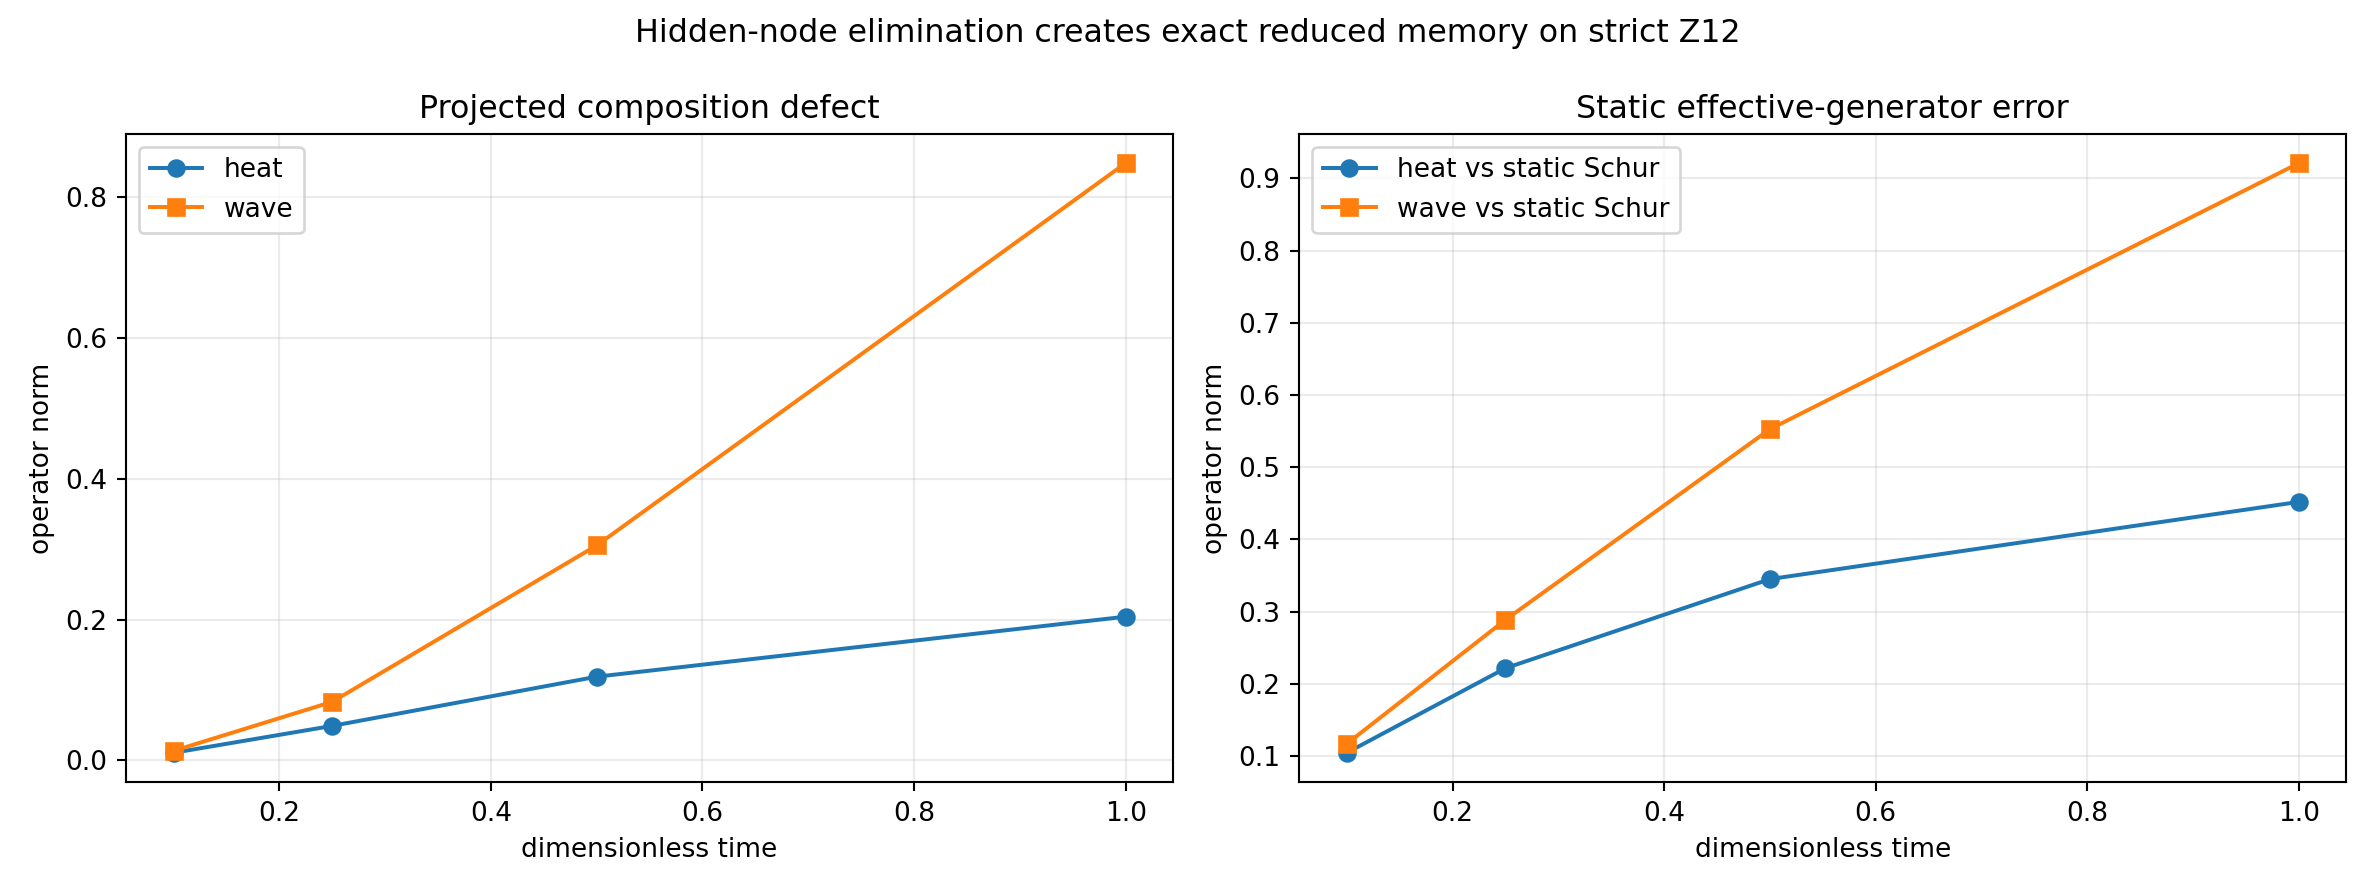
\includegraphics[width=0.97\textwidth]{FIN_Nadsoliton_Puzzle_Atlas_Figures/dynamic_schur_memory.png}
\caption{Composition defect of reduced propagators and the error incurred by replacing dynamic reduction with one static Schur generator.}
\end{figure}

\section{Significance}

\begin{itemize}
\item 
\textbf{\statusProven{}} Fractal elimination of degrees of freedom generates memory even when the full dynamics is a homogeneous semigroup or group.

\item 
\textbf{\statusProven{}} Wave and diffusion dynamics share the same block-resolvent object but produce different time records.

\item 
\textbf{\statusModerate{}} \(\Sigma_E(z)\) is a strong candidate for the missing mathematical interface between compression, environment, and apparatus.

\item 
\textbf{\statusRefuted{}} Static \(A_{\rm Schur}\) is not an exact generator of the entire reduced dynamics for the audited partition.

\item 
\textbf{\statusRefuted{}} Memory after reduction does not establish a fundamental arrow of time or a conscious observer.

\end{itemize}

\chapter{"Shadow shapes": new intuitions}

\section{The missing object may be a noncommutativity defect}

Many unresolved components share the form

\[
\text{reduce first, then evolve}
\neq
\text{evolve first, then reduce}.
\]

The defect of this commutation is an observable shadow of hidden degrees of freedom. \textbf{\statusStrong{}}

\section{The observer is a section of a process, not an added substance}

Mathematically, an observer may mean:

\begin{itemize}
\item 
a selected subalgebra of accessible observables;

\item 
a projection \(P\);

\item 
a set of permitted instruments;

\item 
a rule for recording multitime data.

\end{itemize}

This does not introduce an "informational layer beneath the nadsoliton." It is an operational section of nadsoliton states. \textbf{\statusModerate{}}

\section{\texorpdfstring{\(C_\chi\) and the chiral bispectrum receive the same resource type}{C\_ and the chiral bispectrum receive the same resource type}}

Both are odd under inversion and reverse sign with the preparation. They may belong to a common class of monotone asymmetry receivers. \textbf{\statusModerate{}} Neither is thereby a sign selector.

\section{Different observables see different harmonics}

The blindness of \(C_1\) when \(C_\chi\neq0\) is a general tomographic lesson. One current or one interference image does not identify the full operator. \textbf{\statusProven{}}

\section{Static and dynamic self-similarity are distinct hypotheses}

Failure of strict to close under a static Schur map does not rule out a simpler structure for the family \(\Sigma^{(n)}(z)\). This is a new, well-typed hypothesis. \textbf{\statusSpeculative{}}

\section{Scale can be relative, but an experiment requires an anchor}

Spectral ratios are identifiable without an absolute clock; absolute energies and times are not. \textbf{\statusProven{}} A projective fingerprint can be tested first, but a physical theory still requires calibration.

\section{Information geometry may be real without being spacetime}

The heat kernel gives a diffusion metric and scale hierarchy but does not establish Lorentz signature or spacetime geometry. \textbf{\statusProven{}}

\section{The most defensible architecture still has two additional packages}

\begin{itemize}
\item 
\(W_0\): the strict dimensionless information-operator core;

\item 
an operational/\allowbreak{}conversion package: preparation, scale, instrument, environment, and record;

\item 
a sector package: an explicit orientation/\allowbreak{}branch resource.

\end{itemize}

Dynamic self-energy may enrich the first interface, but it does not remove the other two packages.

\chapter{Falsification of analogies}

\begin{center}
\begingroup\small
\setlength{\tabcolsep}{2.5pt}
\renewcommand{\arraystretch}{1.16}
\begin{longtable}{@{}p{0.224\textwidth}p{0.369\textwidth}p{0.267\textwidth}@{}}
\toprule
\textbf{Tempting analogy} & \textbf{Destructive test} & \textbf{Verdict} \\
\midrule
\endhead
strict = Yukawa propagator & test whether the inverse and local operator are derived rather than fitted & conditional reconstruction only \\
duality = observer paradox & same generator but different instruments and records & no mathematical paradox \\
Schur = RG fixed point & test closure of the strict family & \statusRefuted{} in the audited realization \\
chiral current = selector & phase inversion gives an equally valid opposite sign & \statusRefuted{} as a source \\
bifurcation = unique choice & symmetric law produces a pair of branches & \statusRefuted{} without bias \\
entropy = energy & no temperature, Hamiltonian, or apparatus reset & \statusRefuted{} without additional axioms \\
diffusion distance = physical length & generator rescaling changes calibration & \statusRefuted{} as an SI metre \\
process tensor = ontology & depends on accessible interventions and system/\allowbreak{}environment split & operational description only \\
\(\Sigma(z)\) = new fundamental field & changing the projection changes \(\Sigma\) & \statusRefuted{} as projection independent \\
graphical resemblance = theory equivalence & no operation- and observable-preserving maps & \statusRefuted{} methodologically \\
\bottomrule
\end{longtable}
\endgroup
\end{center}

\chapter{Twelve subsequent research programs}

\section{Program 243 --- Dynamic Schur theorem for arbitrary partitions}

Prove conditions for positivity and complete monotonicity of \(\Sigma_E(z)\), minimality of the memory realization, and a necessary-and-sufficient criterion for exactly Markovian reduction.

\textbf{Probability of a valuable result:} 0.90.\\
\textbf{Success criterion:} an if-and-only-if theorem plus tests of every nonisomorphic \(Z_{12}\) partition.

\section{Program 244 --- Common analytic self-energy of wave and diffusion}

Build one resolvent package and derive its limits

\[
z>0\quad\text{(heat)},\qquad z=\epsilon-i\omega\quad\text{(wave)}.
\]

\textbf{Probability:} 0.82.\\
\textbf{Risk:} confusing analytic continuation with physical Wick rotation without axioms.

\section{Program 245 --- Identifiability of the observed/\allowbreak{}hidden partition}

Determine whether distinct \(E/H\) splits can generate the same process on \(E\), and construct equivalence classes of minimal realizations.

\textbf{Probability:} 0.80.

\section{\texorpdfstring{Program 246 --- \(C_\chi\) as a twist-response theorem}{Program 246 --- C\_ as a twist-response theorem}}

Define a flux-twisted family \(A(\theta)\) and test

\[
C_\chi\stackrel{?}{=}
\left.\frac{d}{d\theta}
\operatorname{Tr}[\rho A(\theta)]
\right|_{\theta=0}
\]

with correct treatment of \(d=6\), gauge covariance, and orientation reversal.

\textbf{Probability:} 0.86.

\section{Program 247 --- Current-harmonic tomography}

Measure

\[
C_d=\sum_xJ(x\to x+d),\qquad d=1,\ldots,5
\]

instead of only \(C_1\), and determine the minimum preparations and observables required to identify the chiral part of a state.

\textbf{Probability:} 0.84.

\section{Program 248 --- Asymmetry-resource budget}

Compare \(C_\chi\), the chiral bispectrum, and the earlier \(\Lambda(\rho,A)\) as receivers of one resource. Prove bounds of the form

\[
|\langle C\rangle_\rho|\leq M_R(\rho)\|C\|_\infty.
\]

\textbf{Probability:} 0.78.\\
\textbf{Boundary:} classification of receivers, not a new selector.

\section{Program 249 --- Fractal cascade of memory}

Iterate layer elimination and study

\[
\Sigma^{(n+1)}(z)=\mathcal F(\Sigma^{(n)}(z)).
\]

Seek a fixed point in operator-function space rather than in the existing static-kernel family.

\textbf{Probability:} 0.62.\\
\textbf{Reward:} high; this would be the proper dynamic version of fractal compression.

\section{Program 250 --- Process-memory test with a complete record}

Extend P240--P242 by an intervention at an intermediate time. Distinguish:

\begin{itemize}
\item 
a single semigroup on 12 states;

\item 
a static six-state model;

\item 
the exact six-state process with memory.

\end{itemize}

\textbf{Probability:} 0.75, laboratory dependent.

\section{Program 251 --- False positives of the spectral fingerprint}

Generate broad Laplacian classes and determine how many non-FIN operators pass the projective-spectrum, semigroup, harmonic-current, and prescribed-reduction memory tests.

\textbf{Probability:} 0.88.

\section{Program 252 --- Stability of heat/\allowbreak{}Fisher geometry under reduction}

Compare diffusion distances and the Fisher metric before and after Schur reduction and dynamic reduction.

\textbf{Probability:} 0.73.\\
\textbf{Boundary:} the result remains dimensionless.

\section{Program 253 --- Can dynamic self-energy generate strict damping?}

Treat this as one new bridge atom, not a repetition of a generic legacy-to-strict audit. Test whether elimination of a declared self-similar layer can generate

\[
(1+\beta d^{9/5})^{-1}
\]

without encoding \(9/5\) in the input.

\textbf{Probability:} 0.38.\\
\textbf{Stop rule:} one explicit ansatz; do not enlarge the family after a no-go.

\section{Program 254 --- Blind hidden-excursion test}

Preregister

\[
T_E(2\tau)-T_E(\tau)^2
=PT(\tau)QT(\tau)P^\ast
\]

and measure both sides from independent records.

\textbf{Probability:} 0.70.\\
\textbf{Value:} directly distinguishes static reduction from a process with memory.

\chapter{Research priority}

\begin{center}
\begingroup\small
\setlength{\tabcolsep}{2.5pt}
\renewcommand{\arraystretch}{1.16}
\begin{longtable}{@{}p{0.235\textwidth}p{0.205\textwidth}p{0.420\textwidth}@{}}
\toprule
\textbf{Priority} & \textbf{Program} & \textbf{Reason} \\
\midrule
\endhead
1 & P243 & highest theorem confidence and immediate clarification of reduction \\
2 & P246 & completes simulator methodology and current definition \\
3 & P247 & prevents blindness to all but one harmonic \\
4 & P244 & formally joins wave and diffusion after reduction \\
5 & P251 & measures specificity of the complete FIN fingerprint \\
6 & P245 & determines what can actually be inferred about an "environment" \\
7 & P250 & moves the result into an operational multitime process \\
8 & P248 & orders chiral receivers without pretending to find a source \\
9 & P252 & tests information geometry \\
10 & P254 & supplies a falsifiable memory experiment \\
11 & P249 & high reward, greater risk \\
12 & P253 & most difficult and most vulnerable to target coding \\
\bottomrule
\end{longtable}
\endgroup
\end{center}

\chapter{What this report does not claim}

The report does not export:

\begin{itemize}
\item 
a strict selector or discharge of QW-2191;

\item 
a canonical scale of length, time, mass, energy, or action;

\item 
closure of the legacy-to-strict bridge;

\item 
transfer of legacy physical roles;

\item 
\(L_{\rm total}\), the Standard Model, GR, or a ToE;

\item 
evidence that any laboratory realizes FIN;

\item 
evidence that projection-generated memory is fundamental memory in nature.

\end{itemize}

\chapter{Shortest interpretation surviving falsification}

The strict FIN core is a finite positive spectral generator whose different functions produce coherent propagation, diffusion, a Green function, and a quadratic action. Chirality belongs to resources of states or operations, not to the radial generator. When some degrees of freedom are hidden---as naturally occurs both in fractal compression and for an observer---the exact shadow of the full theory is not another static kernel but a frequency-dependent self-energy and a process with memory.

This is currently the richest mathematical picture obtained by assembling the puzzles. It is more precise and more testable than the claim that one plot merely "looks like" a familiar phenomenon.

\chapter{Comparative literature}

\begin{enumerate}
\item 
Dörfler, F.; Bullo, F., \emph{Kron Reduction of Graphs with Applications to Electrical Networks}, \href{https://arxiv.org/abs/1102.2950}{https:/\allowbreak{}/\allowbreak{}arxiv.org/\allowbreak{}abs/\allowbreak{}1102.2950}.

\item 
Lin, Y. T.; Tian, Y.; Anghel, M.; Livescu, D., \emph{Data-driven learning for the Mori--Zwanzig formalism}, \href{https://arxiv.org/abs/2101.05873}{https:/\allowbreak{}/\allowbreak{}arxiv.org/\allowbreak{}abs/\allowbreak{}2101.05873}.

\item 
Pollock, F. A. et al., \emph{Non-Markovian quantum processes: complete framework and efficient characterisation}, \href{https://arxiv.org/abs/1512.00589}{https:/\allowbreak{}/\allowbreak{}arxiv.org/\allowbreak{}abs/\allowbreak{}1512.00589}.

\item 
Marvian, I.; Spekkens, R. W., \emph{Modes of asymmetry}, \href{https://arxiv.org/abs/1312.0680}{https:/\allowbreak{}/\allowbreak{}arxiv.org/\allowbreak{}abs/\allowbreak{}1312.0680}.

\item 
Shuman, D. I. et al., \emph{The Emerging Field of Signal Processing on Graphs}, \href{https://arxiv.org/abs/1211.0053}{https:/\allowbreak{}/\allowbreak{}arxiv.org/\allowbreak{}abs/\allowbreak{}1211.0053}.

\item 
Coifman, R. R.; Lafon, S., \emph{Diffusion maps}, \href{https://doi.org/10.1016/j.acha.2006.04.006}{https:/\allowbreak{}/\allowbreak{}doi.org/\allowbreak{}10.1016/\allowbreak{}j.acha.2006.04.006}.

\item 
Chamseddine, A. H.; Connes, A., \emph{The Spectral Action Principle}, \href{https://arxiv.org/abs/hep-th/9606001}{https:/\allowbreak{}/\allowbreak{}arxiv.org/\allowbreak{}abs/\allowbreak{}hep-th/\allowbreak{}9606001}.

\end{enumerate}

\chapter{Reproducible artifacts}

\begin{itemize}
\item 
Z12 sim.html --- corrected interactive simulator.

\item 
audit\_z12\_sim.py --- independent mathematical audit.

\item 
Z12\_sim\_methodological\_audit.json --- results of 15 tests.

\item 
fin\_nadsoliton\_puzzle\_atlas.py --- atlas and dynamic-Schur study.

\item 
FIN\_Nadsoliton\_Puzzle\_Atlas\_All\_Singles.csv --- 180 comparisons.

\item 
FIN\_Nadsoliton\_Puzzle\_Atlas\_All\_Pairs.csv --- 990 comparisons.

\item 
FIN\_Nadsoliton\_Puzzle\_Atlas\_Results.json --- values and candidate ranking.

\item 
FIN\_Nadsoliton\_Puzzle\_Atlas\_Figures/\allowbreak{} --- figures.

\end{itemize}


\clearpage
\chapter*{Reproduction certificate}
\addcontentsline{toc}{chapter}{Reproduction certificate}
\begin{Verbatim}[fontsize=\small]
python3 audit_z12_sim.py
MPLCONFIGDIR=/tmp/matplotlib-puzzle \
python3 fin_nadsoliton_puzzle_atlas.py
\end{Verbatim}
Expected Z12 audit result: 15/15 tests passed. Atlas scores are search
heuristics; operator theorems are verified with separate residuals.
\end{document}
